\documentclass[aspectratio=169,10pt]{beamer} % or 14 or 17 or 20

\usepackage{tikz,pgf,lmodern,textpos,hyperref,graphicx,booktabs,appendixnumberbeamer,cleveref,fancybox,multicol}
\usepackage{pgfcalendar,pgfornament,svg,subfiles,chronosys,cancel,xcolor,color,nth,datenumber,xparse,fp,stackengine,makecell}
  
\usetikzlibrary{positioning}
\usepackage[outline]{contour}
\usepackage[citestyle=authoryear-comp,backend=bibtex]{biblatex}
\usepackage[export]{adjustbox}
\usepackage[en-US]{datetime2}
\usepackage[normalem]{ulem}
\bibliography{references}
\usetheme{metropolis}



%!TEX Root = ./presentation.tex

\definecolor{Blue}{HTML}{00548f}
\definecolor{Cardinal Red}{HTML}{8c1515}
\definecolor{White}{HTML}{ffffff}
\definecolor{Cool Grey}{HTML}{4d4f53}
\definecolor{Black}{HTML}{2e2d29}
\definecolor{Bright Red}{HTML}{B1040E}
\definecolor{Dark Red}{HTML}{820000}
\definecolor{Chocolate}{HTML}{2F2424}
\definecolor{Stone}{HTML}{544948}
\definecolor{Fog}{HTML}{F4F4F4}
\definecolor{Light Sandstone}{HTML}{F9F6EF}
\definecolor{Sandstone}{HTML}{d2c295}
\definecolor{Warm Grey}{HTML}{3f3c30}
\definecolor{Beige}{HTML}{9d9573}
\definecolor{Light Sage}{HTML}{c7d1c5}
\definecolor{Clay}{HTML}{5f574f}
\definecolor{Cloud}{HTML}{dad7cb}
\definecolor{Driftwood}{HTML}{b6b1a9}
\definecolor{Stone}{HTML}{928b81}
\definecolor{Sandhill}{HTML}{b3995d}
\definecolor{Palo Alto}{HTML}{175e54}
\definecolor{Teal}{HTML}{00505c}
\definecolor{Purple}{HTML}{53284f}
\definecolor{Redwood}{HTML}{8d3c1e}
\definecolor{Brown}{HTML}{5e3032}
\definecolor{Sky}{HTML}{0098db}
\definecolor{Lagunita}{HTML}{007c92}
\definecolor{Mint}{HTML}{009b76}
\definecolor{Gold}{HTML}{b26f16}
\definecolor{Sun}{HTML}{eaab00}
\definecolor{Poppy}{HTML}{e98300}

\definecolor{USF Green}{HTML}{00543C}
\definecolor{USF Gold}{HTML}{FDBB30}
\definecolor{USF Grey}{HTML}{919194}
% \definecolor{USF }{HTML}{e98300}


\setbeamercolor{normal text}{fg=Black,bg=White}
\hypersetup{colorlinks,linkcolor=USF Green,urlcolor=USF Green,citecolor=USF Green}
% \setbeamercolor{frametitle}{bg=Cardinal Red, fg=Blue}


\setbeamercolor{palette primary}{bg=Fog, fg=USF Green}
\setbeamercolor{palette secondary}{bg=USF Green, fg=Fog}
\setbeamercolor{frametitle}{bg=Fog,fg=USF Green}

% \setbeamercolor{section title}{fg=Dark Red, bg=Fog}
\setbeamercolor{alerted text}{fg=USF Green}

\newcommand{\soutthick}[1]{%
    \renewcommand{\ULthickness}{2.4pt}%
       \sout{#1}%
    \renewcommand{\ULthickness}{.4pt}% Resetting to ulem default
}


  \setbeamercolor{normal text}{%
    fg=Cool Grey,
    bg=White
  }

\setbeamercolor{palette primary}{fg=Fog, bg=Dark Red}
\setbeamercolor{palette secondary}{bg=Dark Red, bg=Fog}
\setbeamercovered{transparent}
% \setbeamercolor{background canvas}{bg=Fog}
\setbeamercolor{frametitle}{bg=Dark Red,fg=Fog}
\hypersetup{colorlinks,linkcolor=Blue,urlcolor=Blue,citecolor=Blue}
\setbeamercolor{alerted text}{fg=Bright Red}
\setbeamertemplate{caption}{\insertcaption}


\setsansfont[BoldFont={Source Sans Pro Bold},
              Numbers={OldStyle}]{Source Sans Pro}
\setmainfont[BoldFont={Source Serif Pro Semibold},
              Numbers={OldStyle}]{Source Serif Pro}
\setmonofont{Source Code Pro}


\metroset{titleformat=smallcaps,numbering=none}


\newenvironment{mystepwiseitemize}{\begin{itemize}[<+-| alert@+>]}{\end{itemize}}







\title{some interesting CHI papers}
\subtitle{that you might not have seen}
\author{Ali Alkhatib}
\institute[RWF]{Reading With Friends}

\date{May 13, 2019}





\newcommand{\onlyinsubfile}[1]{#1}
\newcommand{\notinsubfile}[1]{}
\begin{document}
\renewcommand{\onlyinsubfile}[1]{}
\renewcommand{\notinsubfile}[1]{#1}
\begin{frame}
\titlepage
\end{frame} 


% \def\stackalignment{l}
% \def\stacktype{S}


\begin{frame}{roadmap thing}
     \tableofcontents
\end{frame}


\section[Witchcraft and HCI: Morality, Modernity, and Postcolonial Computing in Rural Bangladesh]{Witchcraft and HCI: Morality, Modernity, and Postcolonial Computing in Rural Bangladesh {\scriptsize \color{Black} by \textbf{Sharifa Sultana} \& \textbf{Syed Ishtiaque Ahmed}}}

\begin{frame}[t] % \frametitle{Witchcraft and HCI}
\includegraphics[width=\textwidth]{pdfs/witchcraft.pdf}
\end{frame}

\begin{frame}\frametitle{why i liked it}
    \begin{itemize}
      \item brings in anthro stuff
      \item interviews witches
      \item shows how witches in rural india use technology and understand/navigate the world with it:

      {\itshape
      \vspace{1em}
       ``we found the witches in Jessore using modern communication technologies including television, satellite channels, mobile phones, and the Internet.''
      
      \vspace{1em}
      
      ``\dots witchcraft can provide HCI researchers with examples and inspirations for making a deeper engagement with various moral values, designing with their similarities and differences, emphasizing on communal relationship, and neutralizing radicalism by using other local sources of power.''
      }
    \end{itemize}
\end{frame}


\section[``They Don’t Leave Us Alone Anywhere We Go'': Gender and Digital Abuse in South Asia]{``They Don’t Leave Us Alone Anywhere We Go'': Gender and Digital Abuse in South Asia {\scriptsize \color{Black} by \textbf{Nithya Sambasivan}, \textbf{Amna Batool}, \textbf{Nova Ahmed}, \textbf{Tara Matthews}, \textbf{Kurt Thomas}, \textbf{Laura Sanely Gaytán-Lugo}, \textbf{David Nemer}, \textbf{Elie Bursztein}, \textbf{Elizabeth Churchill}, \& \textbf{Sunny Consolvo}}}

\begin{frame}[t] % \frametitle{``They Don’t Leave Us Alone Anywhere We Go''}
\includegraphics[width=\textwidth]{pdfs/they_dont_leave_us_alone.pdf}
\end{frame}

\begin{frame}\frametitle{why i liked it}
    \begin{itemize}
      \item talks about distinct forms of abuse online:
      \begin{enumerate}
        \item cyberstalking
        \item impersonation
        \item personal content leakages (doxxing)
      \end{enumerate}
    \end{itemize}
\end{frame}

\begin{frame}
\includegraphics[page=8,width=\textwidth]{pdfs/they_dont_leave_us_alone.pdf}
\end{frame}


\section[Guerilla Warfare and the Use of New (and Some Old) Technology: Lessons from FARC's Armed Struggle in Colombia]{Guerilla Warfare and the Use of New (and Some Old) Technology: Lessons from FARC's Armed Struggle in Colombia {\scriptsize \color{Black} by \textbf{Débora de Castro Leal},  \textbf{Max Krüger },  \textbf{Kaoru Misaki },  \textbf{David Randall}, \& \textbf{Volker Wulf}}}

\begin{frame}[t] % \frametitle{Guerilla Warfare and the Use of New (and Some Old) Technology}
\includegraphics[width=\textwidth]{pdfs/guerilla_warfare.pdf}
\end{frame}

\begin{frame}\frametitle{why i liked it}
    \begin{itemize}
      \item interviewed former FARC guerillas
      \item talks about how tech gets used in this conflict
      \begin{enumerate}
        \item telecom (radio, paper, computer encryption)
        \item sensing, localization, targeting technologies (and storing food off-site to avoid being detected)
        \item mass media (radio, internet, etc\dots)
        \item learning tools
      \end{enumerate}
      \item a bit about the stuff that you have to do to do fieldwork

      {\itshape
      \vspace{0.5em}

      ``The specific camp our study is set in is located 3-4 hours by car away from the closest city, only reachable by 4x4 jeep.''

      \vspace{0.5em}

      ``In total, 114 pages were collected, and the authors interacted with more than 50 people. Due to the unstable situation, both researchers and inhabitants of the ETCR were forced to treat their interactions flexibly. Some information was obtained in single conversations lasting several hours, some in repeated interactions, some lasted only a few minutes. Author one and five speak intermediate Spanish, and all interactions were conducted in Spanish.''
      }
    \end{itemize}
\end{frame}


\section[Ethical Dimensions of Visualization Research]{Ethical Dimensions of Visualization Research {\scriptsize \color{Black} by \textbf{Michael Correll}}}

\begin{frame}[t] % \frametitle{Ethical Dimensions of Visualization Research}
\includegraphics[width=\textwidth]{pdfs/ethical_dimensions.pdf}
\end{frame}

\begin{frame}\frametitle{why i liked it (but it's not in the papers :\textbackslash~)}
    \includegraphics[width=\textwidth]{figures/IMG_9728.jpeg}
\end{frame}

\begin{frame}\frametitle{why i liked it (more seriously)}
    \begin{itemize}
      \item makes a strong, succinct point in line with \citeauthor{bowker2000sorting} {\small (\citetitle{bowker2000sorting})}
      \item argues for more attention to \strong{the provenance} of data
      \item makes a number of recommendations (way more details in the paper):
      \begin{enumerate}
        \begin{columns}
        \begin{column}{0.1\textwidth}
        \end{column}
        \begin{column}{0.4\textwidth}
        \item visualize hidden labor
        \item visualize hidden uncertainty
        \item visualize hidden impacts
        \item encourage ``small data''
        \item anthropomorphize data
        \end{column}
        \begin{column}{0.4\textwidth}
        \item obfuscate data to protect privacy
        \item support data ``due process''
        \item act as data advocates
        \item pressure or slow unethical analytical behavior
        \end{column}
        \end{columns}
      \end{enumerate}
    \end{itemize}
\end{frame}


\section[Technologies for Social Justice: Lessons from Sex Workers on the Front Lines]{Technologies for Social Justice: Lessons from Sex Workers on the Front Lines {\scriptsize \color{Black} by \textbf{Angelika Strohmayer}, \textbf{Jenn Clamen}, \& \textbf{Mary Laing}}}

\begin{frame}[t] % \frametitle{Technologies for Social Justice}
\includegraphics[width=\textwidth]{pdfs/technologies_for_social_justice.pdf}
\end{frame}

\begin{frame}\frametitle{why i liked it}
    \begin{itemize}
      \item who's talking about sex work at CHI? seriously
      \item talks about ``abnormal justice''~(\cite{doi:10.1086/589478}):
      \begin{enumerate}
        \item What does justice look like?
        \item How can we move towards this idea of justice?
        \item And who decides what the answers to these two questions are?
      \end{enumerate}
      {\itshape
      \vspace{1em}
      ``there are instances where institutional ideas of justice are incongruent with what those affected by these frameworks consider `just' – Fraser calls this  `\strong{abnormal justice}' '' (emphasis added)
      \vspace{1em}
      }
      \item discusses ``The List'' as an instantiation of ``abnormal justice''
    \end{itemize}
\end{frame}


\section[``I Bought This for Me to Look More Ordinary'': A Study of Blind People Doing Online Shopping]{``I Bought This for Me to Look More Ordinary'': A Study of Blind People Doing Online Shopping {\scriptsize \color{Black} by \textbf{Guanhong Liu}, \textbf{Xianghua Ding}, \textbf{Chun Yu}, \textbf{Lan Gao}, \textbf{Xingyu Chi}, \& \textbf{Yuanchun Shi}}}

\begin{frame}[t] % \frametitle{``I Bought This for Me to Look More Ordinary''}
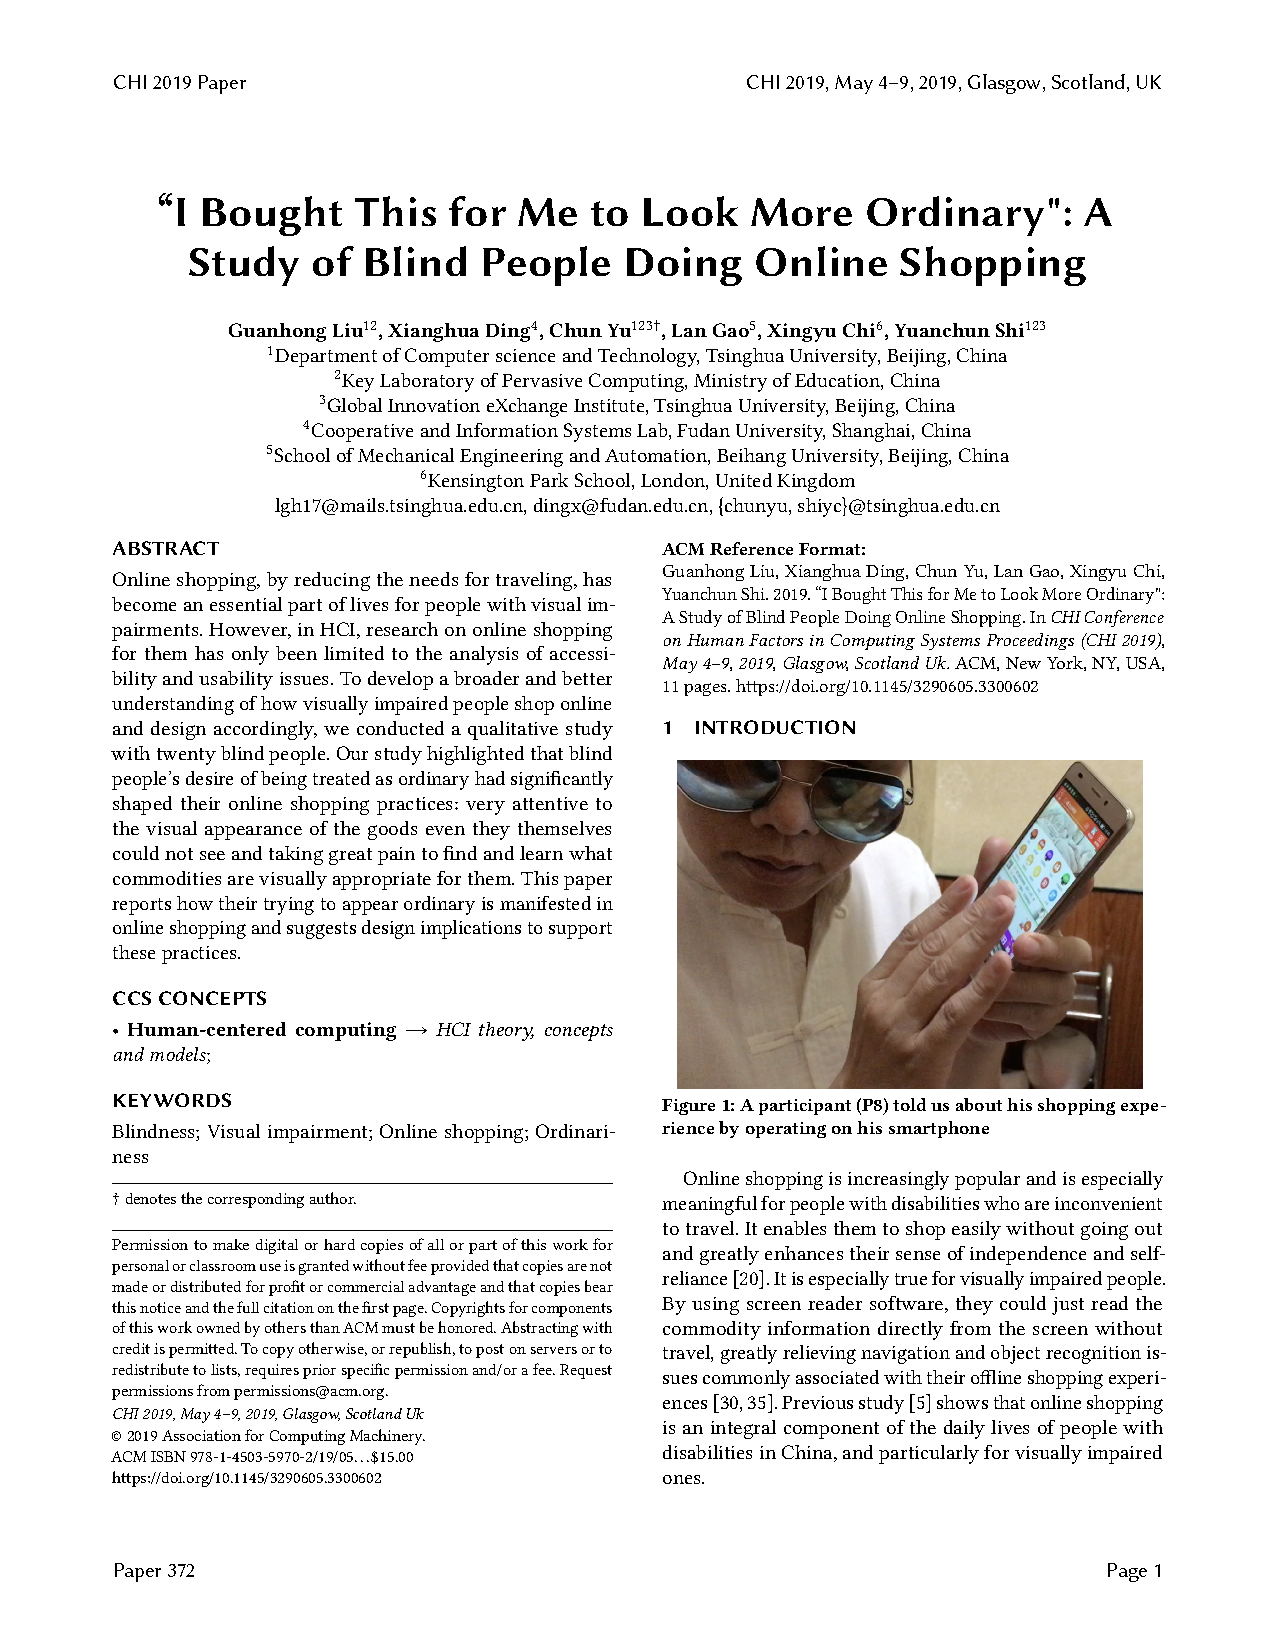
\includegraphics[width=\textwidth]{pdfs/i_bought_this_to_look_more_ordinary.pdf}
\end{frame}

\begin{frame}\frametitle{why i liked it}
    \begin{itemize}
    \item pointed out that people actively avoid disclosing, even in online shopping experience
    {\itshape
\vspace{1em}

``for online shopping, our participants tried to avoid asking customer service for help when it came to questions with blind features (questions that could be solved through looking at pictures, such as what a product looks like), also for the sake of ordinariness''

\vspace{1em}
}
      % \item i didn't know much about how people who experience disabilities may be willing to go to great lengths to avoid having to disclose that to others if they can help it (e.g. reluctance to disclose to customer service representative, asking about how something looks)
      \item made me reflect on whether you can trust the \strong{passively} collected data to reveal this stuff (or more precisely, how I should make more effort to actively seek out this stuff if i'm designing something)
    \end{itemize}
\end{frame}




\end{document} 